\documentclass[preprint,12pt]{elsarticle}
\usepackage{amsmath,amssymb}
\usepackage{graphicx}
\usepackage{booktabs}
\usepackage[version=4]{mhchem}
\usepackage{siunitx}
\usepackage{xcolor}
\usepackage{url}
\usepackage{lineno}
\journal{Water Research}

\begin{document}

\begin{frontmatter}

\title{Testing effort sets the water-quality criterion:
a support-dependent artefact that regulatory screening narrows but does not remove}

\author[snu]{Jeongyun Kim\fnref{eq}}
\author[cbdri]{Jin Yoo\fnref{eq}}
\author[cbdri]{Ku Kang\corref{cor}}
\ead{bisu9082@mnd.go.kr}
\affiliation[snu]{organization={Department of Chemical and Biological Engineering, Seoul National University},
 city={Seoul}, country={Republic of Korea}}
\affiliation[cbdri]{organization={CBRN Defense Research Institute}, country={Republic of Korea}}
\cortext[cor]{Corresponding author.}
\fntext[eq]{These authors contributed equally to this work.}

\begin{abstract}
Aquatic water-quality criteria are anchored on an extreme of the available
toxicity data: the lowest reported no-effect concentration, or the fifth
percentile of a species sensitivity distribution. Both move as the evidence
behind them grows, and they move for different reasons. From 4744 curated
ECOTOX records covering 87 per- and polyfluoroalkyl substances (PFAS) we derive
criteria under seven conventions and join them to measured surface-water
concentrations from 1180 United States stations. On the six substances every
convention can assess from the same 10\,362 measurements, the fraction of
samples exceeding the criterion runs from 98.8\,\% to zero on derivation choice
alone. Reproducing the screen agencies apply --- apical endpoints, chronic
exposure durations, active ingredient, species mean chronic values, a
log-normal fit --- brings the two routes they actually use from 78.6\,\% against
4.6\,\% to 14.8\,\% against 4.6\,\%, but leaves both as dependent on testing
effort as before (Spearman $\rho = -0.590$ and $-0.681$). Screening reconciles
the routes without removing the bias they share. Two channels produce it:
minimum-anchored conventions inherit the sample-size behaviour of an order
statistic, while the fifth percentile moves because the fitted spread widens
with testing breadth, which supplies 63\,\% of its slope. Across all 4757 ECOTOX
chemicals with freshwater acute data, equalising sampling depth and controlling
within-chemical spread leaves a partial correlation of $-0.004$: the two
channels account for essentially the whole association. Perfluorooctanoic and
perfluoroheptanoic acid, at the same 810 stations, receive fully screened
criteria 523-fold apart, behind which stand 313 and 6 apical chronic records.
\end{abstract}

\begin{keyword}
PFAS \sep water quality criteria \sep predicted no-effect concentration \sep
species sensitivity distribution \sep data availability bias \sep ECOTOX
\end{keyword}

\end{frontmatter}

\linenumbers
\sloppy

\section{Introduction}

Per- and polyfluoroalkyl substances (PFAS) are a routine feature of surface
water, detectable at the majority of sampled United States stations
\cite{salvatore2023pfasoccur}. Managing that exposure requires a water-quality
criterion: a single concentration standing in for the sensitivity of an entire
aquatic community. Every major framework arrives at that number by taking an
extreme of whatever toxicity data happen to exist --- the European guidance by
dividing the lowest reliable no-observed-effect concentration by a factor
reflecting trophic coverage \cite{echa2008r10}, the United States by a final
chronic value from the four lowest genus means, Canada and Australia by the
fifth percentile of a species sensitivity distribution (SSD)
\cite{posthuma2019ssd}. The methods differ in detail and agree in structure:
the criterion is a low order statistic of a sample whose size nobody controls.

The resulting variability is recognised. Thirteen groups deriving a no-effect
concentration for one substance from one dossier produced a spread in which the
derivation step was a leading source \cite{hoondert2014pnecvar}; sample-size
guidance has been formalised \cite{belanger2019ssdsize}, minimum data
requirements evaluated empirically \cite{hiki2018mindata}, and assessment
factors revisited against species count \cite{iwasaki2022afssd}. That
literature asks how precise the fifth percentile is. We ask whether its
expected value moves, and whether the movement reaches decisions about real
water.

For a fixed distribution of species sensitivities the expectation of the sample
minimum falls as the sample grows: a substance studied in forty species will on
average present a lower extreme than the same substance studied in four, even
if the two are equally toxic. Where testing effort is distributed unevenly, as
it emphatically is for PFAS, the derived criterion acquires a component that
reflects attention rather than hazard.

The PFAS case is unusually sharp. Perfluorooctanoic acid (PFOA) and
perfluorooctane sulfonate (PFOS) have been the subject of restriction,
litigation and drinking-water standards for two decades
\cite{kwiatkowski2020class}, with dedicated criteria derivations going back as
far \cite{giesy2011pfospnec}. Their homologues and the ethers and telomer
products that replaced them occur in the same rivers at comparable
concentrations and have been tested a fraction as often
\cite{ankley2021pfasrisk}; whether the replacements are less hazardous remains
contested \cite{brandsma2022genxsub}, and that question is asked of criteria
derived from very different amounts of evidence. Compilations such as ECOTOX
\cite{olker2022ecotox} reproduce the imbalance faithfully, and models trained
on them to fill the gaps inherit it \cite{khan2019ecotoxqsar,
liang2025datagaps, sarkar2026pfasqsar}. The hazard is familiar from
biodiversity records, where the apparent distribution of a taxon partly maps
where people looked \cite{yang2015samplingbias}.

That the extreme-anchored route is conservative is understood, and the
conservatism is under active revision: Ding et al.\ \cite{ding2026af} argue
that the assessment-factor method systematically overestimates aquatic risk and
set out ways to temper it, treating the conservatism as a bias of roughly fixed
size to be corrected by better-calibrated factors. Our results complicate that
programme. The conservatism is not fixed; it varies with how much the substance
has been studied, so no uniform adjustment can remove it, and a factor
calibrated on data-rich compounds will mis-calibrate data-poor ones in a
predictable direction.

Two questions follow. Whether the effort dependence is real has been addressed
in general terms for sample-size effects on SSD percentiles
\cite{newman2000ssd, aldenberg2000hcunc, zhao2016ssdmodel}. Whether it matters
--- whether the choice of convention changes which real water bodies are judged
at risk, and whether the screening agencies perform, which database-driven
analyses usually skip, removes it --- has not, to our knowledge, been asked.

This paper answers the second question. We derive PFAS criteria from one
curated ECOTOX extract under seven conventions, from the mechanical minimum
used in recent data-driven work to a reproduction of the regulatory screen and
SSD, and join each to 20\,682 measured concentrations from 1180 United States
stations. The exceedance fraction ranges over orders of magnitude; the screen
reaches the right numerical range and reconciles the derivation routes with
each other without removing their shared dependence on effort; the reason is
mechanical, identifiable, and different for the two families of convention.

\section{Materials and methods}

\subsection{Aquatic toxicity data}

We used the ECOTOX ASCII release of 15 September 2026 \cite{olker2022ecotox}.
Aquatic tests on fluorinated substances were extracted at the result level,
retaining the eight endpoint codes used by the source curation and discarding
censored values; species identity and taxonomic group were joined through
\textsf{test\_id} and \textsf{species\_number}, both joins complete, yielding
151 species. Substances were collapsed to parent structures, so that acid,
anionic and salt forms of one PFAS are one substance, by retaining the largest
fluorine-containing fragment of each recorded SMILES and neutralising it with
the RDKit \textsf{Uncharger} \cite{rdkit}. After deduplication on test
identifier, endpoint, concentration and unit this yields 4744 records over 87
parent substances. Unit conversions, endpoint codes and the censoring rule are
set out in full in the supporting information.

\subsection{Reproduction gates}

Three assertions guard the analysis and run before any result is computed: the
rebuilt parent-level table must reproduce a previously deposited 87-substance
table exactly; the per-substance minimum must be recoverable from the
result-level table for all 87; and the generalisation set below must reproduce a
deposited 4757-chemical table. All three pass. Their purpose is to ensure that
differences reported between conventions are differences of convention and not
of extraction. Details, and the two defects that made the second gate fail at
first pass, are in the supporting information.

\subsection{Seven derivation conventions}

A predicted no-effect concentration (PNEC) was computed as
\begin{equation}
\mathrm{PNEC} = \frac{10^{\,\ell}\times 10^{3}}{\mathrm{AF}}\quad
[\si{\micro\gram\per\litre}],
\end{equation}
where $\ell$ is a log-toxicity in \si{\milli\gram\per\litre} chosen by the
convention and AF an assessment factor. With $\mathrm{AF}=1000$ throughout,
\textbf{C1} takes the lowest value over all endpoints and records --- the target
variable of recent structure-based PFAS screening work and the reference case
here; \textbf{C2} repeats C1 with \textsf{LOEC} records removed, isolating an
endpoint type that reports a concentration at which an effect \emph{was}
observed and is therefore inadmissible as a no-effect basis; \textbf{C3} takes
the lowest acute value (\textsf{LC50}, \textsf{EC50}, \textsf{IC50});
\textbf{C4} the median acute value over records; and \textbf{C5} the median over
species of each species' median acute value. \textbf{C6} takes the lowest
chronic \textsf{NOEC} with an EU Technical Guidance factor set by chronic
trophic coverage --- 10 for three or more levels, 50 for two, 100 for one
\cite{echa2008r10}; \textbf{C6$'$} applies the same factor to the lowest
\emph{apical} chronic \textsf{NOEC} of adequate exposure duration, which is
what the guidance actually specifies and which we report alongside C6
throughout. \textbf{C7} is the regulatory-style screen below.

\subsection{Exposure-duration criteria}

ECOTOX assigns \textsf{NOEC} and \textsf{LOEC} codes without regard to exposure
duration, so a chronic endpoint code does not by itself identify a chronic
test: 23.8\,\% of the records carrying a chronic endpoint code in our extract
have exposure durations of 96 hours or less. Wherever a convention is described
below as chronic we therefore additionally require a taxon-appropriate
duration --- at least 72 hours for algae and aquatic plants, at least 168 hours
(seven days) for invertebrates, fish and amphibians --- and report the
unfiltered result alongside it. Records whose duration cannot be resolved to
hours are excluded from the filtered variant. This requirement reduces the
number of substances supporting a species sensitivity distribution from 16 to
13 and leaves the effort dependence essentially unchanged
($\rho = -0.691 \rightarrow -0.681$), which is reported in Section~\ref{sec:screen}.

\subsection{The regulatory-style screen (C7)}

Regulatory derivations do not use a compilation as deposited; they screen it. We
implemented that screen explicitly and auditably: chronic endpoints only
(\textsf{NOEC}, \textsf{NOEL}, \textsf{MATC}, \textsf{EC10}), apical effects
only (mortality, growth, reproduction, development, population), active
ingredient only. Gene-expression, biochemical, enzymatic, hormonal,
behavioural, histological, cellular and accumulation endpoints are excluded, as
in criteria derivation. Admitting \textsf{EC10} extends the source endpoint set
deliberately, since chronic derivations prefer a regression-based effect
concentration and the substitution shifts the fifth percentile in a
dataset-dependent direction \cite{iwasaki2015noecec10}. Surviving records were
reduced to species mean chronic values by geometric mean within species; with
five or more species a log-normal SSD was fitted and its fifth percentile (HC5)
taken with no further factor, following the Canadian and Australian protocols,
and with fewer the lowest species mean divided by 10 is reported instead.

\subsection{Generalisation set}

To test whether the behaviour is specific to PFAS or to our substance selection,
the same question was put to the whole of ECOTOX: all acute freshwater records
extracted under the rules above, giving 106\,095 records on 4757 chemicals of
all structural classes. Sampling depth was then equalised. For each depth
$k \in \{3,5,10,20,50\}$, every chemical with at least $k$ records contributes
$k$ records drawn without replacement over 200 draws, the statistic is
recomputed, and its correlation with the full record count measured. The
difference between the correlation at full depth and at equal depth is the part
attributable to how much the chemical has been tested rather than to how toxic
it is.

\subsection{Measured surface-water concentrations}

Measured concentrations came from the Water Quality Portal, aggregating the
USGS National Water Information System and the EPA Water Quality Exchange
\cite{wqp2026}. The PFAS characteristic-name vocabulary was enumerated from
the portal's code service (139 names) and results requested for all of them,
sample medium water, site types stream and lake, reservoir or impoundment,
from 1 January 2015; full query parameters are in the supporting information.

Records were retained if they carried a unit of \si{\nano\gram\per\litre} or
\si{\micro\gram\per\litre}, a positive value and no non-detection flag;
percent-recovery controls, isotopically labelled surrogates and records
reporting zero under a non-detect flag were removed. This leaves 22\,255
detected concentrations, so every exceedance fraction is conditional on
detection; the all-results fractions in the supporting information move C1
from 76.5\,\% to 24.8\,\% and C7b from 0.78\,\% to 0.34\,\%, leaving the
ordering unchanged.

Each name was mapped to a CAS number with the structure taken from the ECOTOX
substance file rather than the mapping table, so the correspondence is
independently checkable, and names were collapsed to parents by the rule used
for the toxicity data. The 66 names with detected data resolve to 40 CAS
numbers, 18 of which have no aquatic toxicity record and admit no criterion;
the rest join to 20\,682 measurements of 22 parent substances at 1180
stations, 99.6\,\% of them collected from 2019 onward.

\subsection{Model experiment}

Random forests (150 trees) were cross-validated over five folds on Morgan
fingerprints of the 4311 broad-set chemicals with a parsable SMILES, with the
minimum acute value, the median acute value and the record count as alternative
targets, and out-of-fold predictions evaluated within strata of record count. A
further pair of fits used targets with the linear trend on $\log_{10}$(records)
removed. Settings are in the supporting information.

\subsection{Risk quotients and statistics}

A risk quotient is the measured concentration divided by the derived PNEC; a
sample exceeds when the quotient exceeds one and a station exceeds when any of
its samples does. Association between testing effort, taken as $\log_{10}$ of
the number of curated records, and the derived criterion was measured by
Spearman's $\rho$ with 95\,\% confidence intervals from 4000 bootstrap
resamples. Derived criteria were compared with official freshwater
aquatic-life values: the United States 2024 final chronic criteria
\cite{epa2024pfosalc, epa2024pfoaalc}, the European direct-toxicity annual
average standard \cite{eu2013directive, ruffle2024criteria}, the Australian
default guideline values \cite{anzg2018pfos} and the Canadian federal guideline
\cite{eccc2018feqgpfos}. Note that the binding European standard for PFOS of
\SI{0.65}{\nano\gram\per\litre} derives from secondary poisoning and human fish
consumption, not direct aquatic toxicity \cite{eu2013directive}, and is
therefore not the comparator for a PNEC built from aquatic endpoints; the
direct-toxicity component of \SI{230}{\nano\gram\per\litre} is
\cite{ruffle2024criteria}.

SSD fit diagnostics, sensitivity of the effort correlation to distributional
form and minimum species count, the name-to-structure mapping, the
assessment-factor decomposition and the all-results exceedance fractions are in
the supporting information; all code and derived tables are available
(Section~\ref{sec:data}).

\section{Results}

\subsection{What the compilation contains}

The 4744 curated records are dominated by hypothesis-test endpoints: 1918
\textsf{NOEC} and 1811 \textsf{LOEC} values against 953 acute median-effect
values. Because C1 takes a minimum over all endpoints, a
concentration at which an effect \emph{was} observed can become the basis of a
no-effect criterion: for PFOA the lowest \textsf{NOEC} and the lowest
\textsf{LOEC} are the same \SI{1}{\nano\gram\per\litre} in \emph{Danio
rerio}. That pair is a physiological and a biochemical response over 166 hours,
neither apical nor of chronic duration; zebrafish exposures at this level are
reported in the literature \cite{hagenaars2017pfoalow}, so the values are not
data-entry errors, but they are exactly what the screen in
Section~\ref{sec:screen} is meant to exclude. What disqualifies them is not
their magnitude but that unscreened they enter a pool from which a minimum is
taken and divided by an acute-calibrated factor.

The effect types matter more. Gene expression (3501 result rows) is the most frequent reported effect, ahead of biochemistry (1613) and
enzyme activity (867), while the apical effects regulatory derivation retains
account for 29.8\,\% of rows. The imbalance runs with effort: substances with
fewer than 50 records are 60.7\,\% apical by median, those with 200 or more
21.6\,\%. Heavily studied PFAS are studied not with more apical tests but with
more mechanistic ones.

\subsection{The derivation convention spans eight orders of magnitude}

Table~\ref{tab:ladder} gives the result. The conventions do not all reach the
same substances --- C1 assesses 22 of those measured, the SSD only six --- so
applying each to every substance it can assess, as the left block does,
confounds the derivation choice with which substances can be assessed at all.
The right block removes that confound, restricting every convention to the six
substances and 10\,362 measurements common to all. The spread widens rather
than narrows: on identical data the fraction of samples exceeding the
criterion falls from 98.8\,\% under C1 to zero under C5, and the median
criterion moves eight orders of magnitude. Statements below are made on the
common subset unless noted.

The widest contrast involves C1, which no agency would defend: it pools
\textsf{LOEC} values with acute median-effect concentrations and divides by a
single acute-calibrated factor. The result does not depend on it. Comparing only
the two routes agencies do use --- the fully screened European route C6$'$ and
the regulatory SSD C7b --- gives \SI{34.2}{} against
\SI{5770}{\nano\gram\per\litre} on the common subset, 14.8\,\% of samples
against 4.6\,\% and 46.1\,\% of stations against 17.9\,\%, with both
effort-dependent ($\rho = -0.590$ and $-0.681$). Screening narrows the
disagreement between the two routes by an order of magnitude --- unscreened, C6
gives 78.6\,\% against the same 4.6\,\% --- without touching the dependence
they share. C1 is retained
because it is the target variable of published screening work, not because the
argument needs it. Removing \textsf{LOEC} records, which is methodologically
required, moves exceedance only from 76.5\,\% to 76.0\,\%: the error is real but
it is not the driver. Restricting to a single endpoint type matters far more, C3
lifting the median criterion by nearly five orders of magnitude relative to C1.

\begin{table}[t]
\centering
\footnotesize
\setlength{\tabcolsep}{3.5pt}
\caption{Derived criteria and exceedance under seven conventions. The left block applies each convention to every substance it can assess; the right block restricts all conventions to the six substances and 10\,362 measurements that every convention can assess, so that only the derivation choice differs. PNEC is the median across substances, not across measurements.}
\label{tab:ladder}
\begin{tabular}{@{}ll rrr rrr@{}}
\toprule
& & \multicolumn{3}{c}{own substance set} & \multicolumn{3}{c}{common subset ($n=6$)}\\
\cmidrule(lr){3-5}\cmidrule(lr){6-8}
& convention & subs. & PNEC & samp. & PNEC & samp. & stat.\\
& & & (\si{\nano\gram\per\litre}) & (\%) & (\si{\nano\gram\per\litre}) & (\%) & (\%)\\
\midrule
C1 & lowest value, all endpoints & 22 & 4.44 & 76.50 & \num{7.50e-03} & 98.80 & 100.00\\
C3 & lowest acute value & 18 & 1\,730 & 22.70 & 1\,490 & 39.44 & 92.11\\
C5 & median acute, species-resolved & 18 & \num{5.42e+04} & 0.11 & \num{1.80e+05} & 0.00 & 0.00\\
C6 & lowest chronic NOEC $+$ AF & 18 & 15.8 & 55.36 & 0.7 & 78.59 & 99.64\\
C6$'$ & as C6, apical $+$ chronic & 15 & 100 & 7.84 & 34.2 & 14.84 & 46.10\\
C7a & lowest apical SMCV / 10 & 15 & 961 & 6.85 & 218 & 13.43 & 46.01\\
C7b & SSD fifth percentile & 6 & 5\,770 & 4.62 & 5\,770 & 4.62 & 17.85\\
\bottomrule
\end{tabular}
\end{table}




\subsection{The regulatory screen reaches the right range}

C7 is the first convention that lands where official criteria live. Its SSD
fifth percentile for PFOS is \SI{4738}{\nano\gram\per\litre} against the
Canadian federal guideline of \SI{6800}{\nano\gram\per\litre}
\cite{eccc2018feqgpfos}, itself an SSD fifth percentile: a ratio of 0.70
between two independent applications of one method to two separately assembled
dossiers. That is the closest of five available comparisons and reporting it
alone would overstate the agreement: our value is 19 times the United States
2024 criterion (\SI{250}{\nano\gram\per\litre}), 21 times the direct-toxicity
component of the EU standard (\SI{230}{\nano\gram\per\litre}), and 10 and 520
times the Australian 95\,\% and 99\,\% default guideline values. Part of that
spread is protection policy rather than derivation --- the Australian pair is
one distribution read at two percentiles --- but not all of it, and the United
States procedure extrapolates from four genus means rather than fitting a
distribution at all. For PFOA
the HC5 is \SI{9516}{\nano\gram\per\litre} against the United States 2024
criterion of \SI{1e5}{\nano\gram\per\litre} \cite{epa2024pfoaalc}, a factor of
ten low. C1, by comparison, is low by 5.4 orders of magnitude for PFOS and 8.0
for PFOA. Official values for PFOS themselves span
\SIrange{9.1}{6800}{\nano\gram\per\litre} across four authorities, so agreement
to within an order of magnitude is agreement to within the regulators' own
spread. Independent derivations predating the official criteria agree: a
freshwater PNEC for PFOS of \SI{25}{\micro\gram\per\litre}
\cite{giesy2011pfospnec} and criteria for both compounds from a curated
literature set \cite{qi2014pfoscriteria} bracket our C7 percentiles.
Fig.~\ref{fig:official} places every convention against the official values.

\begin{figure}[t]
\centering
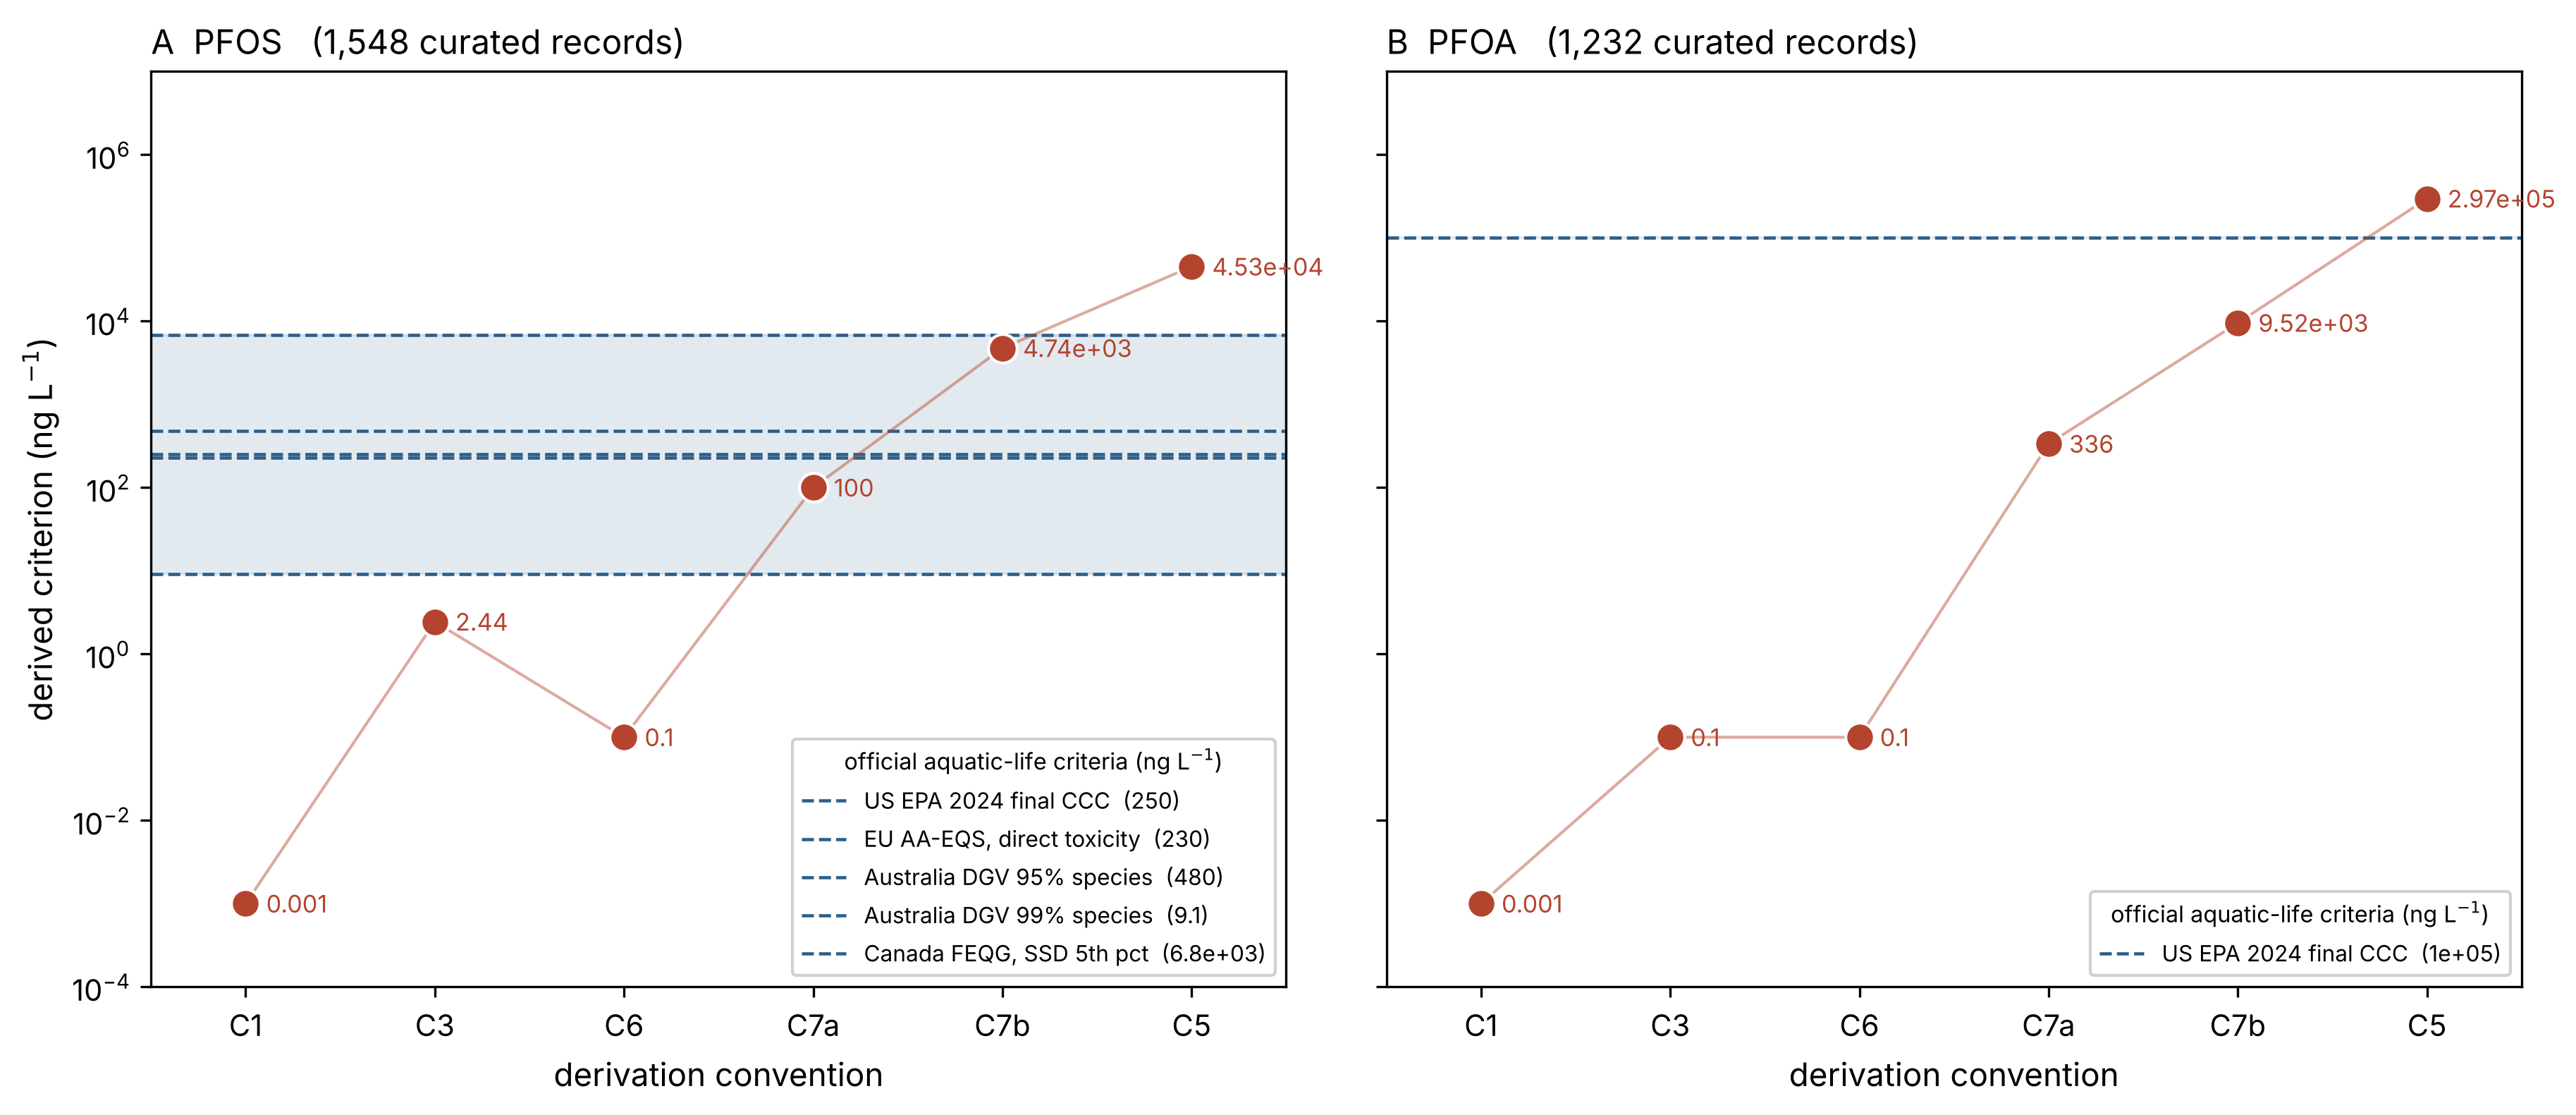
\includegraphics[width=\textwidth]{fig_04_official.png}
\caption{Derived criteria for (A) PFOS and (B) PFOA under each convention,
against official freshwater aquatic-life values. The shaded band in (A) spans
the four authorities. Only the screened conventions reach the regulatory range;
the convention used in published screening work sits five to eight orders of
magnitude below every official value.}
\label{fig:official}
\end{figure}

\subsection{It does not remove the effort dependence}\label{sec:screen}

Fig.~\ref{fig:effort}A is the central result. The rank correlation between
$\log_{10}$ records and the derived criterion is $\rho = -0.783$
(CI $[-0.903, -0.586]$) for C1; after the full regulatory screen it is
$-0.787$ (CI $[-0.887, -0.624]$) for the lowest apical chronic species mean and
$-0.691$ (CI $[-0.940, -0.306]$) for the SSD fifth percentile, with the European
guidance route C6 at $-0.706$ (CI $[-0.856, -0.479]$). Screening the data to the
standard agencies apply leaves the correlation where it was.

One convention shows no detectable effort dependence: the species-resolved acute
median C5, at $\rho = +0.115$ (CI $[-0.240, +0.424]$). We state this as a
failure to detect rather than evidence of independence --- with 41 substances
the interval still admits a weak association either way; what it excludes is a
negative correlation stronger than $-0.24$, anything approaching the $-0.69$ to
$-0.79$ of the extreme-anchored conventions. The lowest acute value C3 is
intermediate and unstable with respect to subset ($\rho = -0.196$,
CI $[-0.509, +0.159]$ on the 41 substances common to all conventions;
$\rho = -0.385$, $p = 0.003$, on the full set of 58), and we draw no conclusion
from it.

\begin{figure}[t]
\centering
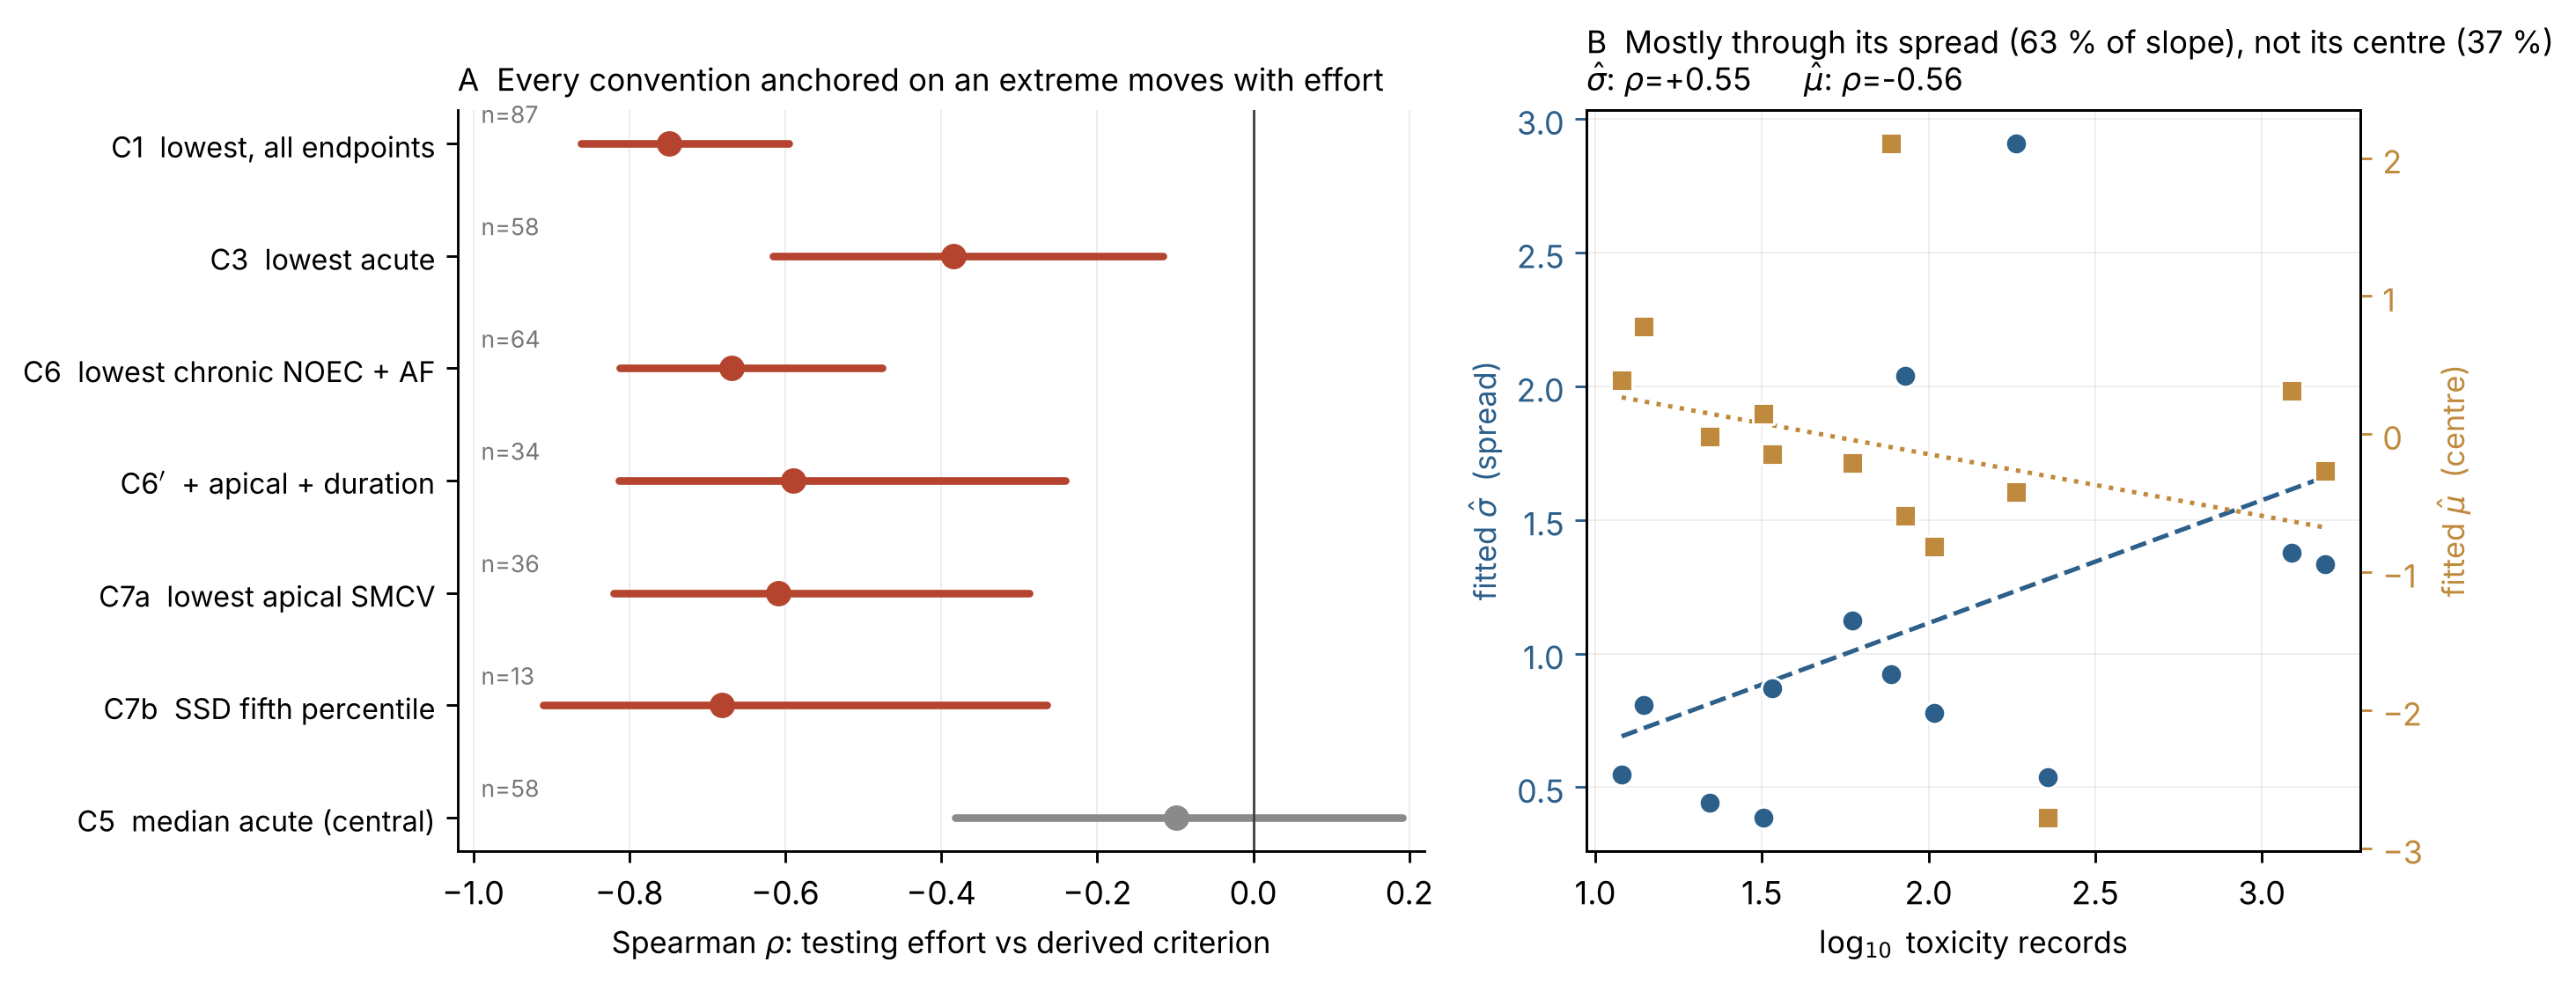
\includegraphics[width=\textwidth]{fig_03_effort.png}
\caption{(A) Spearman correlation between testing effort and the derived
criterion for each convention, with bootstrap 95\,\% confidence intervals from
a fixed seed; red marks an interval excluding zero. (B) The two fitted
parameters of the species sensitivity distribution against record count. The
spread widens with effort and the centre falls; because the fifth percentile
is $\hat{\mu}+z_{0.05}\hat{\sigma}$ and $z_{0.05}$ is negative, the spread
channel supplies 63\,\% of the movement in the HC5.}
\label{fig:effort}
\end{figure}

\subsection{Why: two channels, not one}\label{sec:why}

The mechanism differs between the two families of convention. For those
anchored on a minimum --- C1, C2, C3, C6 and C7a --- it is elementary order
statistics: the expectation of a sample minimum falls as the sample grows, and
the criterion is read off the bottom of whatever happens to be there.

For the species sensitivity distribution it is not. An HC5 computed as
$\hat{\mu} + z_{0.05}\hat{\sigma}$ is a parametric functional, not an order
statistic, and under a correctly specified log-normal model it is a consistent
estimator of a fixed population quantity: asymptotically it should carry no
dependence on sample size at all. Decomposing the observed slope over the 13
duration-filtered substances shows where the dependence enters instead. Both
parameters move: the fitted mean falls by 0.45 per decade of records
($\rho = -0.56$, $p = 0.046$) and the fitted standard deviation rises by 0.46
($\rho = +0.55$, $p = 0.052$). Because $z_{0.05}$ is negative, the spread term
contributes $-0.76$ per decade against the centre's $-0.45$, and the two sum to
the observed $-1.20$: 63\,\% of the movement in the HC5 comes from the fitted
spread widening and 37\,\% from the centre falling. Without the duration
filter the split is sharper still --- the centre's contribution is then not
significant ($\rho = -0.36$, $p = 0.17$) while the spread's is
($\rho = +0.72$, $p = 0.002$), and the spread supplies 69\,\%.

This remains an effort artefact, but a different one. A substance studied more
has been studied across more taxa, endpoints and exposure regimes, and a
distribution fitted to wider evidence is wider; the fifth percentile of a wider
distribution is lower. The number of species surviving the screen does rise
with records ($\rho = +0.756$), but species count does
not predict the HC5 once records are held fixed (partial $\rho = +0.28$,
$p = 0.30$), so the species channel is not the operative one. Calling the whole
effect an extreme-order statistic misidentifies it for the route agencies most
often use, and would send any correction to the wrong place.

A median, being central, does not move with sample size --- and the property
that makes it stable makes it unusable: it offers no protection to the
sensitive tail, and the resulting values would declare essentially all United
States surface water compliant.

\subsection{The assessment factor cannot compensate}

The assessment-factor system is often read as protecting against exactly this:
a substance with little evidence receives a larger factor, so scarcity is paid
for by a more conservative criterion. That reading is generous. The factors
were calibrated for laboratory-to-field and taxon-to-taxon extrapolation, not
for the sample-size behaviour of an extreme estimator, so the arithmetic below
shows what they were never built to do rather than that they fail at it. Over the 62 substances with a chronic
\textsf{NOEC} and an EU Technical Guidance factor, the lowest chronic
\textsf{NOEC} falls by 2.12 $\log_{10}$ units per decade of records
($p = 2\times10^{-10}$) while the factor shrinks it back by only 0.30
($p = 1\times10^{-9}$), so the criterion falls by 1.82 per decade: the factor offsets 14\,\% of the
movement in the underlying endpoint and 86\,\% passes through. The three
slopes satisfy the decomposition exactly, since
$\log C = \log(\text{NOEC}) - \log(\text{AF})$ is an identity; what matters
is not that they sum but how little of the sum the factor carries.

The shortfall is structural, not a matter of calibration. The factor is set by
trophic coverage and takes only the values 10, 50 and 100 here, a range of one
$\log_{10}$ unit, while the effort-attributable movement in the lowest chronic \textsf{NOEC} is
about 6.8 units over the observed range of record counts. A one-decade lever
cannot hold a quantity that moves by nearly seven decades, and no recalibration
of the tiers within the present scheme changes that; a factor that depended on
evidential support rather than on trophic coverage alone could.

\subsection{The artefact is not about PFAS}

Fig.~\ref{fig:broad} puts the same question to 4757 ECOTOX chemicals of all
classes. The minimum acute value falls with record count at $\rho = -0.462$
(CI $[-0.485, -0.438]$), the median far more slowly at $\rho = -0.160$
(CI $[-0.188, -0.132]$). Equalising sampling depth separates the components: at
$k = 5$, over the 1977 chemicals with at least five records, the minimum's
correlation moves from $-0.409$ to $-0.192$ while the median's moves only from
$-0.140$ to $-0.134$. Across every depth tested the depth effect is $-0.16$ to
$-0.24$ on the minimum and $0.00$ to $+0.01$ on the median.

Equalising records does not equalise what the criterion is computed from.
Criteria are read off species, and five records from a deeply-tested chemical
still span more species than five from a shallow one ($\rho = +0.352$).
Repeating the design on species --- drawing $s$ distinct species and using
species means --- removes 50 to 61\,\% of the baseline correlation across
$s = 3$, 5 and 10.

What survives depth equalisation is not a residual hazard signal. The spread of
toxicity values within a chemical rises steeply with how often it has been
tested ($\rho = +0.783$), and that spread accounts for the remainder:
controlling for within-chemical standard deviation, the partial correlation
between record count and the depth-equalised minimum is $-0.004$, and for the
median $-0.039$. The two channels identified in Section~\ref{sec:why} ---
sampling depth for the minimum, fitted spread for the percentile --- between
them exhaust the association. Essentially all of what an extreme-anchored
criterion says about a chemical, beyond what a central statistic says, is a
statement about how much it has been looked at. We cannot exclude that hazard
and attention are genuinely associated in the world, only that no such
association is needed to explain these data.

This also settles a question the PFAS analysis could not. The species-resolved
acute median gave $\rho = +0.115$ on 41 PFAS, reported above as a failure to
detect rather than independence; the broad set shows the true value for a
central statistic to be near $-0.15$, which 41 substances cannot resolve. The
median is not effort-free; it is free of the \emph{depth} component, which is
the component derivation convention controls.

\begin{figure}[t]
\centering
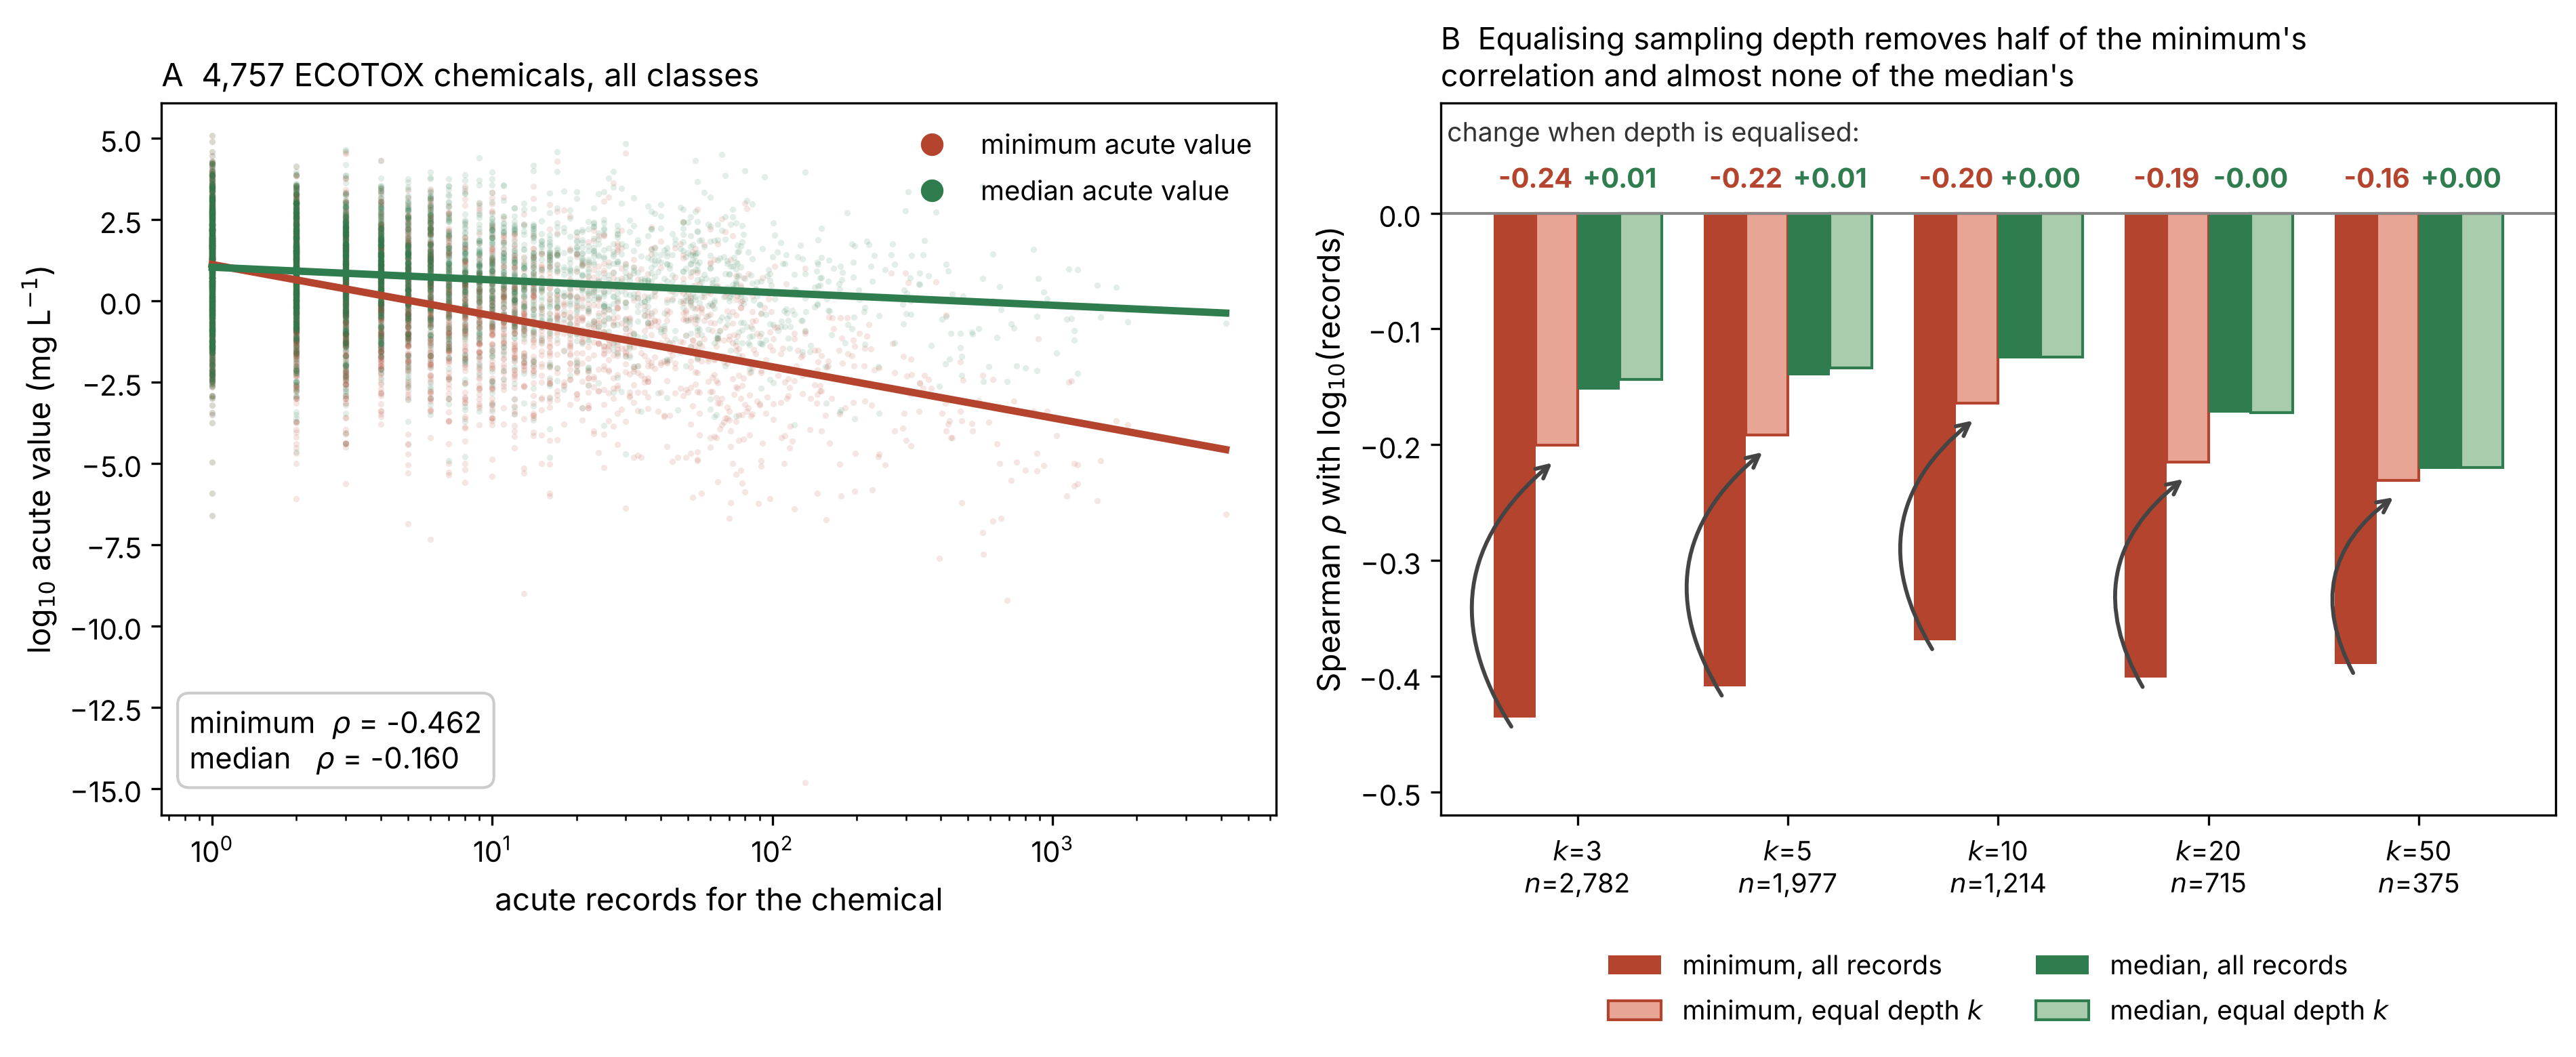
\includegraphics[width=\textwidth]{fig_06_broad.png}
\caption{(A) Minimum and median acute value against the number of acute records,
for all 4757 chemicals in ECOTOX with freshwater acute data. (B) Spearman
correlation with record count at full depth and with sampling depth equalised to
$k$ records per chemical, 200 draws per depth. The figures above each group are
the change when depth is equalised.}
\label{fig:broad}
\end{figure}

\subsection{A matched pair}

Fig.~\ref{fig:pair} isolates the effect from the covariates that might otherwise
explain it. PFOA and perfluoroheptanoic acid (PFHpA) are adjacent homologues
measured at the same 810 stations in the same campaigns, at median \SI{3.9}{}
and \SI{1.7}{\nano\gram\per\litre}, with similar detection frequencies
(58.0\,\% and 55.9\,\%) and the same analytical methods. Under the fully
screened route C6$'$ they receive criteria of \SI{94}{} and
\SI{49200}{\nano\gram\per\litre}, a factor of 523, behind which stand 313
and 6 apical chronic records.

The comparison is stated as a ratio of criteria rather than of exceedance
fractions, deliberately. Unscreened, the same pair gives \SI{0.1}{} against
\SI{144}{\nano\gram\per\litre} and 99.96\,\% against 0.55\,\% of detections
in exceedance; but the PFOA value there rests on the single non-apical
166-hour record discussed above. Screening removes it, raises the PFOA
criterion 940-fold and collapses the exceedance contrast, while leaving the
criterion ratio at 523. The two homologues differ in the quantity of evidence
behind them and in little else the derivation sees; screening changes the size
of the gap, not its direction or its cause.
Supplementary Table~S8 gives the same comparison for all 22 substances.

One feature of that comparison deserves separate statement, because it is the
artefact in its strongest form. Under the full screen an SSD could be fitted for
only six of the 22 substances measured, and those six are among the seven most
heavily studied; no substance outside the top eleven by record count qualifies
under any variant. Whether a substance is eligible for the method that reaches
the regulatory range is itself a function of how much it has been tested, and
the remaining sixteen fall back on an assessment-factor route that
Fig.~\ref{fig:effort}A shows to be at least as effort-dependent. The choice of
method is made for the analyst by the size of the literature, and the methods
available to data-poor substances deviate most from the values regulators
publish for data-rich ones.

\begin{figure}[t]
\centering
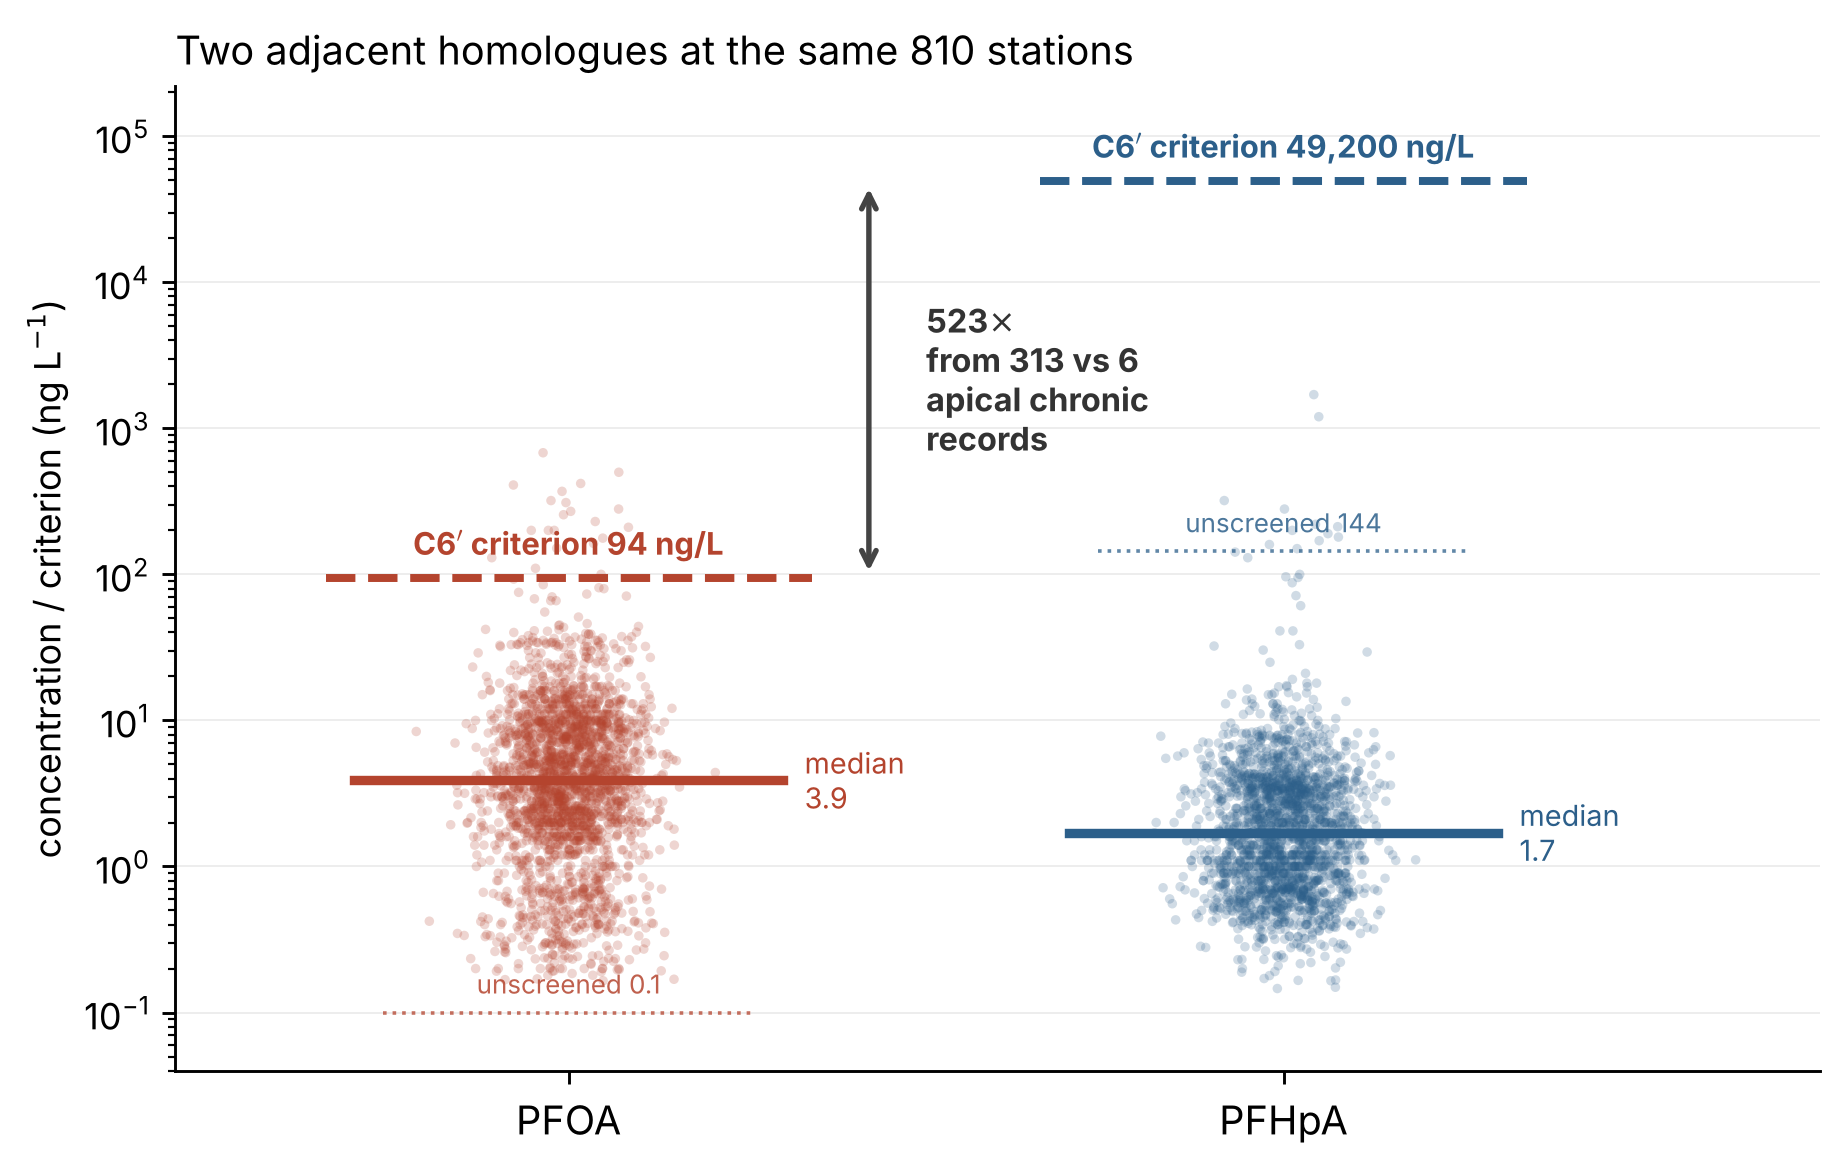
\includegraphics[width=0.66\textwidth]{fig_05_pair.png}
\caption{PFOA and PFHpA measured at the same 810 United States stations, with
the criterion derived for each under the European guidance route. The two are
adjacent homologues present at comparable concentrations; they differ in how
often they have been tested.}
\label{fig:pair}
\end{figure}




\section{Discussion}

\subsection{A structural property, not a curation defect}

It is tempting to read the C1 result as a criticism of careless database use.
The screened experiment removes that reading: applying the screen agencies
apply reproduces one national guideline closely and three others to within one
to two orders of magnitude, and leaves the effort dependence unchanged. The
artefact comes not from poor curation but from anchoring on a
support-dependent statistic, and every current framework anchors on one --- the
lowest NOEC in Europe, the four lowest genus means in the United States, the
fifth percentile in Canada and Australia.

Under current practice, generating more ecotoxicological data on a substance
tends to lower its criterion, independently of whether the new data show it to
be more toxic, and the assessment factor offsets about a seventh of that
movement. A data gap therefore leaves a substance \emph{less} protected under
such a criterion, not more, despite machinery intended to ensure the opposite.

\subsection{A criterion below the analytical floor}

One consequence is operational rather than statistical, and it applies to the
most-studied substances rather than to the median one. Taken across substances,
the median criterion under the published convention is
\SI{4.4}{\nano\gram\per\litre}, which is measurable. For PFOA and PFOS it is
\SI{0.001}{\nano\gram\per\litre}. No detection anywhere in this record falls
below that, the smallest value either substance is reported at is
\SI{0.1}{\nano\gram\per\litre}, and published performance for the methods
that produced these data places reporting limits for the perfluoroalkyl acids
at roughly \SIrange{0.4}{8}{\nano\gram\per\litre} under EPA Method 1633 and
\SIrange{1.4}{16}{\nano\gram\per\litre} under Method 533. The criterion for
the two most-studied PFAS sits two to four orders of magnitude below the
smallest concentration the monitoring that produced this record can report.
Seven of the 22 measured substances have a C1 criterion below their own
smallest detected concentration.

A criterion positioned there cannot be used. Compliance at a non-detecting
station is undetermined, because the reporting limit sits above the criterion,
and compliance at any detecting station is automatically failed; the measurement
carries no information about the decision. This is produced by the same
mechanism as the effort dependence: for the two most-studied PFAS the minimum of
a large mixed-endpoint pool has descended past the range in which the substance
can be observed at all. Past a certain amount of study, a support-dependent
criterion does not merely shift the threshold but moves it out of the measurable
range. That this happens to the best-studied substances and not to the median
one is the point rather than a qualification of it.

\subsection{Implications for criteria setting}

We do not conclude that regulatory criteria are wrong: the agencies' values for
PFOS span a range our reproduction lands inside. The claim is narrower and
harder to dismiss. Two substances with the same true sensitivity distribution
but different amounts of testing receive systematically different criteria, so
wherever criteria are used comparatively --- to rank substances for
restriction, to prioritise monitoring, to choose between replacement
chemistries --- the comparison is partly a comparison of literature sizes. This
bears directly on attempts to recalibrate the assessment-factor method
\cite{ding2026af}: a uniform correction will over-correct the data-poor
substances, whose criteria are least depressed, and under-correct the
data-rich ones. Screening frameworks that rank unregulated contaminants by
integrated hazard face the same exposure \cite{kim2026dualthreat}, as do
risk maps built to show where monitoring coverage is thin
\cite{kang2026dbpcarto}. The replacement question is already contested
toxicologically \cite{brandsma2022genxsub}; we add a procedural reason why a
replacement can look preferable without being so.

\subsection{Does group-based regulation dissolve the problem?}

The field's own answer to data scarcity in PFAS is not to derive a lenient
criterion for each data-poor substance but to stop deriving substance by
substance. The European universal PFAS restriction proposal abandons
substance-level derivation explicitly, and the Drinking Water Directive sets a
sum-of-twenty parameter in which no individual substance carries a value of its
own \cite{oecd2021pfas, patlewicz2019category}. If substance-level criteria are
going away, it is fair to ask why their support dependence matters.

It matters for three reasons our data speak to. A group criterion has to be
anchored somewhere, and in practice on the best-studied members: here PFOA and
PFOS carry 1232 and 1548 records against a median of 30 across the other
twenty, so a group value inherited from them inherits the channel of
Section~\ref{sec:why}. Read-across likewise selects its source by data
availability, which is to say it selects the substance whose criterion has
descended furthest. And grouping does not remove the comparative uses:
deciding which homologue to restrict first, or whether a replacement is
acceptable, remains a comparison across very unequal support. HFPO-DA,
introduced to replace PFOA, carries 85 records against PFOA's 1232; a
substitution judged on derived criteria will tend to favour whichever
chemistry has been examined less.

The honest framing is also narrower than the one we began with. A data-poor
substance does not usually receive a lenient criterion; it receives no criterion
at all. Of the 22 PFAS measured in United States surface water here, 20 have no
official aquatic criterion, and after the full screen only six support an SSD.
What support dependence changes is not mainly the stringency of the criteria
that get issued but which substances can be assessed at all, and how the few
that can are ranked against each other.

\subsection{Implications for models trained on derived criteria}

A growing literature trains QSAR and machine-learning models to predict aquatic
criteria or lowest-observed toxicity values for untested substances
\cite{khan2019ecotoxqsar, liang2025datagaps}. Such models
inherit the problem in a form their usual metrics do not reveal. Fitting random
forests to the broad set with the minimum acute value as target, we find that
prediction bias runs with testing depth --- under-predicting by 0.66
$\log_{10}$ units for chemicals with a single record and over-predicting by
2.33 for those with a hundred or more --- while the Spearman correlation within
each stratum stays between 0.57 and 0.63. The ranking survives; the calibration
does not, and for the best-studied chemicals the model places the most
sensitive endpoint two orders of magnitude higher, that is less hazardous, than
the database records. Supplementary Section~S12 reports the experiment in full.
What catches this failure is stratifying performance by each substance's
training support and reporting an error metric sensitive to level rather than
rank; applicability-domain analysis \cite{sahigara2012ad} and
out-of-distribution alerting \cite{kang2026openset} do not, because training
and test sets carry the bias equally.

\subsection{What can be done}

No modification of the statistic on its own solves the problem: a lower
confidence limit on the HC5, which several protocols already use, moves the
correlation only from $-0.691$ to $-0.635$, because protective intent requires
an extreme and the extreme is what moves. Four partial measures follow, in the
order we would attempt them.

First, criteria should be published with the support that produced them: the
number of records, species and trophic levels, and the endpoint composition.
Minimum data requirements exist in most protocols \cite{hiki2018mindata,
belanger2019ssdsize}, but they operate as a threshold to pass rather than a
quantity to report, and a criterion from four species and one from fifty-seven
are not interchangeable. Second, comparative uses should be restricted to
substances of comparable support, or corrected for it. Third, where a substance
is data-poor the assessment-factor route is preferable to an SSD fitted to a
short species list --- not because it is less effort-dependent, since
Fig.~\ref{fig:effort}A shows it is somewhat more so, but because it states its
uncertainty as a number rather than burying it in a tail estimated from five
points; an HC5 fitted to five species carries a 95\,\% confidence interval up
to seven $\log_{10}$ units wide (Supplementary Table~S2). Fourth, and the only
measure addressing the cause rather than its presentation, assessment factors
could be made to depend on evidential support rather than trophic coverage
alone; work recalibrating factors against species count \cite{iwasaki2022afssd}
is the right shape, and the slope reported above gives the magnitude such a
correction would need. Beyond derivation, 18 of the PFAS measured here have no
aquatic toxicity record at all, and generating apical chronic data for the
data-poorest substances that are measured most often would do more than further
refining the statistics applied to the data-richest \cite{kim2026dualthreat}.

\subsection{Limitations}

Comparison with official criteria rests on two substances, because final
freshwater aquatic-life criteria exist only for PFOA and PFOS; twenty of the
twenty-two PFAS found in United States surface water have no official criterion
and eighteen no toxicity record at all. That is part of the picture but limits
external validation, and the European list is expected to widen
\cite{brack2023wfdcomment}.

The generalisation set is acute-only and neither species-resolved nor collapsed
to parent structures. The SSD analysis uses a log-normal fit and a five-species
minimum, both conventional and both generous; several national protocols
require more species and taxonomic coverage we do not impose, and
Supplementary Table~S4 shows that raising the species minimum removes the
variation being measured rather than correcting it. The measurement set is
restricted to United States stream and lake stations, 99.6\,\% of it collected
from 2019 onward, with dissolved and total fractions not separated and
non-detections excluded, so every exceedance fraction is conditional on
detection. We treat the ECOTOX record as given: study-level reliability
scoring, which agencies perform and the deposited fields do not support
\cite{hull2000dataquality}, is the main screen we could not apply.

\section{Conclusions}

Water-quality criteria for PFAS fall as substances are studied more. On the six
substances for which every convention can be applied to the same 10\,362
measurements, the fraction of samples in exceedance runs from 98.8\,\% to zero
across derivation conventions alone. Reproducing the screen that agencies
perform --- apical endpoints, chronic exposure durations, active ingredient,
species mean chronic values, a log-normal distribution --- brings the two routes
agencies actually use much closer to each other, from 78.6\,\% against 4.6\,\%
to 14.8\,\% against 4.6\,\%, but leaves both as dependent on testing effort as
before ($\rho = -0.590$ and $-0.681$). Screening reconciles the routes; it does
not remove the bias they share.

Two channels produce that bias. Minimum-anchored conventions inherit the
sample-size behaviour of an order statistic; the fifth percentile of a species
sensitivity distribution does not, its movement being mostly the fitted spread
widening as a substance is tested across more taxa and conditions, which
accounts for 63\,\% of the slope. Across 4757 ECOTOX chemicals, equalising
sampling depth and controlling for within-chemical spread leaves a partial
correlation of $-0.004$, so the two channels account for essentially the whole
association. We therefore treat this as a structural property of
support-dependent derivation rather than a defect of practice, and recommend
that criteria be reported with the support that produced them and compared
only across substances of comparable support.

\section*{Data availability}
\label{sec:data}
All analysis code, the derived criterion tables, the characteristic-name to
structure mapping with verification formulae, and the exceedance results are
available in a public repository. The underlying toxicity data are the ECOTOX
ASCII release of 15 September 2026 and the measured concentrations are public
records of the Water Quality Portal; neither is redistributed here.

\section*{Declaration of competing interest}
The authors declare that they have no known competing financial interests or
personal relationships that could have appeared to influence the work reported in
this paper.

\section*{Declaration of generative AI and AI-assisted technologies in the
manuscript preparation process}
During the preparation of this work the authors used Anthropic Claude to write
and debug the analysis code, generate the figures from that code, and draft and
revise manuscript text. After using this tool the authors reviewed and edited
the content as needed, independently verified every reported figure against the
deposited data, and take full responsibility for the content of the published
article.

\bibliographystyle{elsarticle-num}
\bibliography{myref}

\end{document}
